\subsection{A Learning Approach to Natural Language Understanding \cite{Pieraccini1994}}

This paper proposes a learning paradigm for the problem of understanding spoken language. The basis of the work is in a formalization of the understanding problem as a communication problem. The resulting understanding algorithm consists in a Viterbi maximization procedure analogous to that commonly used for recognizing speech.

The first step of this paper is to formalize the NLU problem as a \emph{communication problem}. Two assumptions are made in this step: 1) the meaning of a sentence can be expressed by a sequence of basic units $\mM = \mu_1, ..., \mu_{N_M}$, and there is a sequential correspondence between $\mu_j$ and a subsequence of the acoustic observation $A = a_1, ..., a_{N_a}$; 2); 2) the second assumption is to think of the acoustic representation as a version of the original sequence of meaning units corrupted by a noisy channel. Thus for a given acoustic observation $A$, the problem of understanding a sentence can be expressed as finding $\mathop{\max\arg}_\mM P(\mM | A)$.

A simple choice is to define a unit of meaning as a keyword/value pair $m_j = (k_j, v_j)$, where $k_j$ is a conceptual category (e.g. origin, meal) and $v_j$ is the value in the actual sentence (e.g. Boston, breakfast). In what follows we use $W = w_1, ..., w_{N_W}$ to denote the sequence of words, and use $C = c_1, ..., c_{N_W}$ to denote the sequence of concept labels.

Using the Bayesian rule, the formula can be expressed as:
$$\mathop{\max\arg}_{W,C} P(A | W, C) P(W | C) P(C).$$
It is further assumed that:
$$P(w_i | w_{i-1}, ..., w_1, C) = P(w_i | w_{i-1}, ..., w_{i-n+1}, c_i),$$
$$P(c_i | c_{i-1}, ..., c_1) =  P(c_i | c_{i-1}, ..., c_{i-m}).$$
When $n=m=1$, this is equivalent to a first order \emph{hidden Markov model (HMM)}.

\begin{figure}[h]
  \centering
  % Requires \usepackage{graphicx}
  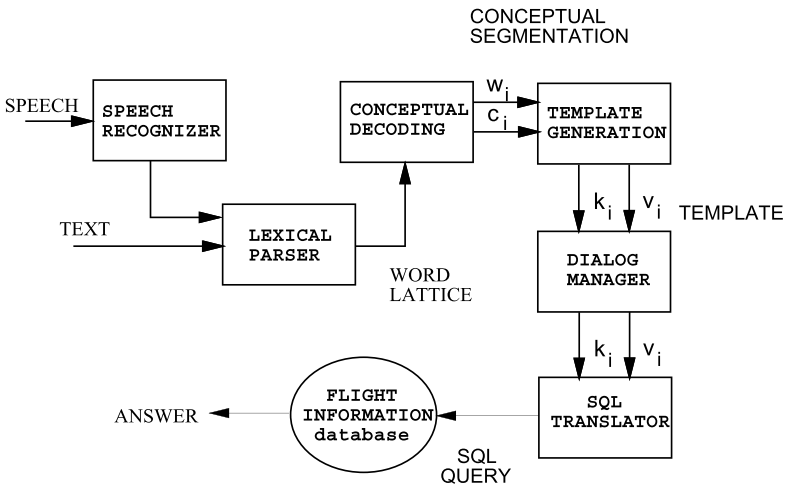
\includegraphics[width=.8\linewidth]{P94-NLU_diag.png}\\
  \caption{Block diagram of the understanding system.}\label{fig:P94-NLU_diag}
\end{figure}

The paper then presents how to implement this idea and apply it to the \emph{ATIS (Air Travel Information System)} corpus. A block diagram of the speech understanding system is presented in Figure \ref{fig:P94-NLU_diag}. Next we will see each of the components in further detail.

In the \emph{conceptual decoding} module, the paper proposes to impose a certain structure to the HMM. It is observed that in a typical sentence there are phases that generally represent the question, a subject and finally a restriction. So the HMM follows this structure to alleviates the problems of the locality of the model and that of concept embedding.

The \emph{lexical parser} dues with different issues related with spoken language, such as the representation of numbers and acronyms. The lexical parser also deletes articles (i.e. THE and A), since they play no role in the conceptual decoding process.

The paper uses the most natural way of \emph{interfacing} the conceptual decoder with a speech recognizer, by directly implementing the maximization of the probability described above. In order to manage the model size, it uses only those words and bigrams that were observed in the training data.

The goal of the \emph{template generator} module is to analyze the conceptual segmentation, and generate the final representation of the meanings. Finally values are assigned to the decoded concepts according to the result of a pattern matching procedure. However, the design of pattern matching tables still requires manual efforts.

The \emph{dialog manager} implements the function of recording the dialog history, and generates proper responses. The simple strategy used in the paper is to keep a current context template, with all the information that has been used. If a concept is mentioned in a new sentence but with a different value, all concepts in the context template at a lower hierarchical level are deleted.

In the experimental study, the proposed system was evaluated on a set of 687 sentences called February 92 test set. The results on the test set from text input account for 68\% of correct answers, 18\% wrong answers and 14\% rejects. When the system was coupled with a speech recognizer through the best first hypothesis, the performance dropped to 52\% of correct answers, 26\% wrong answers and 22\% rejects.
